\documentclass{article}

\usepackage{graphicx}

\begin{document}

\title{Checkpoint}

\section{Experiments and Results}

\subsection{Q-Learning}

\begin{figure}[htp]
\centering
	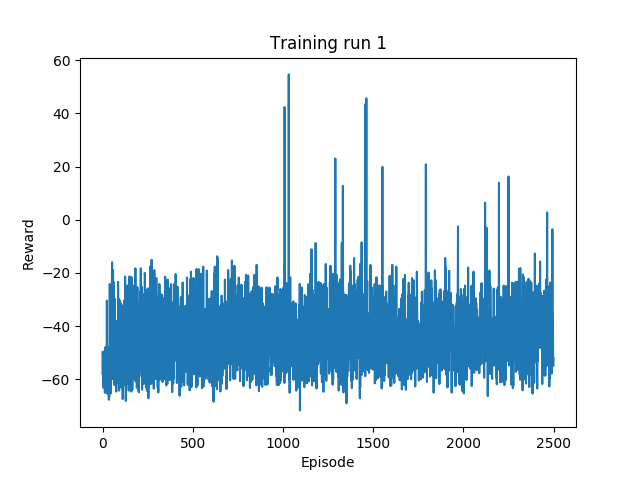
\includegraphics[width=.5\textwidth]{run_1_rewards.png}\hfill
	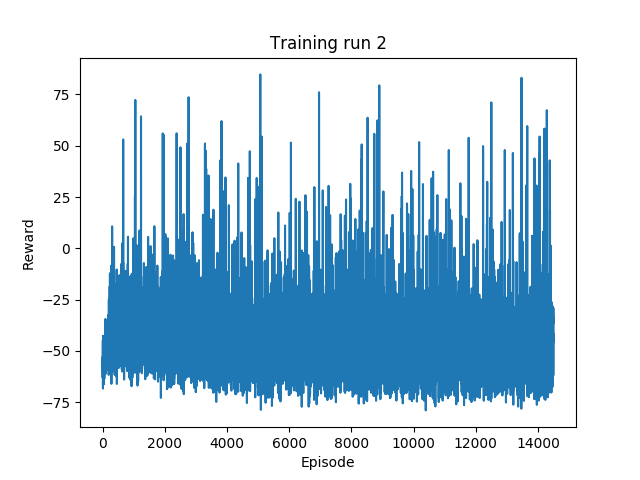
\includegraphics[width=.5\textwidth]{run_2_rewards.png}\hfill
	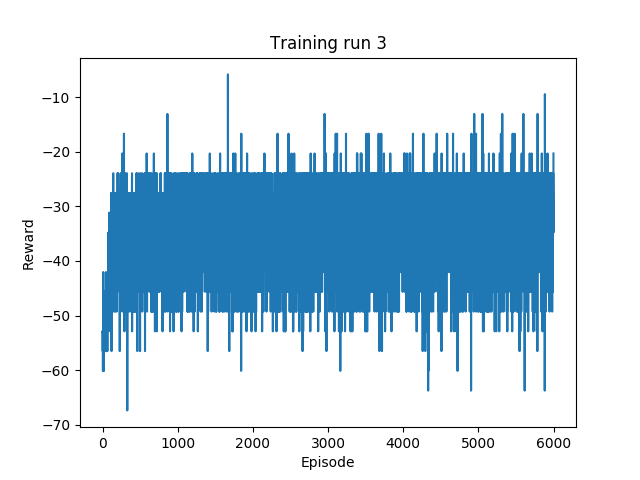
\includegraphics[width=.5\textwidth]{run_3_rewards.png}
\end{figure}


\begin{table}[htp]
\begin{tabular}{|l|l|l|l|l|l|}
\hline
Run & discount rate & learning rate & epsilon & epsilon decay & epsilon floor \\ \hline
1 & 0.99 & 0.01 & 0.05 & N/A & N/A \\ \hline
2 & 0.99 & 0.01 & 0.9 & 0.99 & 0.01 \\ \hline
3 & 0.99 & 0.01 & 0.9 & 0.99 & 0.01 \\ \hline
\end{tabular}
\end{table}

We first ran Q-Learning against the full problem with the state (96x96x4
RGB) given by the environment. This quickly ran out of memory. We
introduced thresholding, binarization, downsampling, and bitpacking to
reduce this memory usage greatly.

Training run 1 was against an 84x96 binary state. The issues we
encountered in this run helped inform subsequent experiments. There is
no learning apparent in its results, as the agent performs similarly to
an agent randomly walking.

We hypothesized that the single largest issue was too large of a state
space. For the second training run, we downsample the state, grabbing
every fourth pixel, to produce a 21x24 state. We also introduce epsilon
decay and an epsilon floor. This training run also performed poorly,
though it does appear to achieve a reward above -20 with more
consistency.

We hypothesized the state space was still too large, so we began working
on a constant track across episodes in training run 3 to reduce it. The
results are more consistent than the previous runs. Even though runs 1
and 2 have some higher rewards, this is a result of ``lucky'' tracks
rather than learning, so this is still an improvement. We also observe
that the car does learn to accelerate down the initial straightaway,
though this learning is reflected poorly in the collected data. This
supports our hypothesis that the state space was too large, as we began
to observe real learning.
A smaller state space means we visit the same states more often, necessitating less exploration and allowing for faster training.

Like Q-learning, training the agent using TD-learning had memory issues with the default state size so we used OpenCV package to preprocess the env generated frame signicantly reducing the overall size. Despite 
\section{Difficulties}

Training is simply too slow, as each episode takes too long.
For simple problems like "go fast in the straightaway," the agent can learn well enough.
But without many more episodes, the car will simply not learn to take the first turn.

\section{Next steps}

We must find a way to let episodes complete quicker, possibly by removing rendering steps. 
Implementing replacing traces can also speed up training. 
A slower epsilon decay may help the car to take turns.
We can downsample further to 12x12 to reduce the state space even more; we can also reduce the action space.
This will speed up learning.
We can introduce a hueristic to guide exploration - on random choice in e-greedy policy, choose to turn left or right based on presence of the track on the left or right side of the screen.

\end{document}
